\chapter{实验三(2):模型并行实验}

\section{实验内容与要点介绍}

\subsection{实验内容与要求}
\subsubsection{实验内容}
\begin{itemize}
    % \item 学习掌握模型并行的原理,并了解常用的模型并行策略
    % \item 实现基于横向和纵向按层划分策略的模型并行
    % \item 分析模型并行方式对模型性能的影响
    \item 了解常用模型划分策略;
    \item 编写相应的算法实现代码进行模型的划分;
    \item 分析不同数据划分方法对模型的影响。
\end{itemize}

\subsubsection{实验要求}
\begin{itemize}
    \item 使用RPC相关API,实现模型并行训练
    \item 将模型拆分成两部分,分别在不同节点(进程)上进行训练
    \item 根据实验结果,分析模型并行对分布式系统性能的影响
    % \item (可选)实现横向划分
\end{itemize}

\subsection{RPC框架介绍}

在本实验中,我们将使用Remote Procedure Call(即RPC)框架,对应于\graylstinline{torch.distributed.rpc}。这个框架中的诸多函数,将帮助我们实现模型划分的训练。但应注意,该框架尚不完全支持CUDA,因此建议本实验在CPU上跑,图\ref{fig:task4-warning-cuda-rpc-not-compatible}为官网截图。
\begin{figure}[htbp]
	\centering
	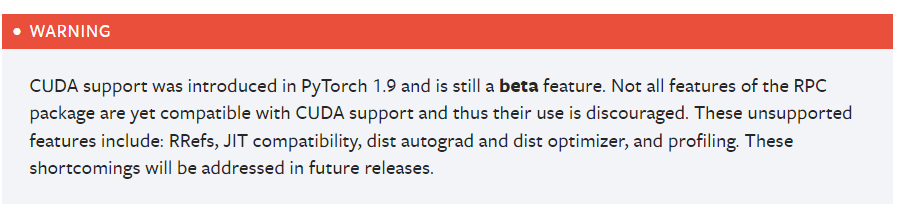
\includegraphics[width=1\textwidth]{figures/task4-warning-cuda-rpc-not-compatible.png}
	\caption{caption:task4-warning-cuda-rpc-not-compatible}
	\label{fig:task4-warning-cuda-rpc-not-compatible}
\end{figure}

\subsubsection{神经网络定义}

假设我们要把一个完整的模型拆分到两个节点上去,每个节点运行一个子模型,即\graylstinline{SubModel1}和\graylstinline{SubModel2}。其工作方式为\graylstinline{SubModel1}作为第一层,\graylstinline{SubModel1}的输出层再链接到\graylstinline{SubModel2}的输入层。

为了实现这一工作方式,我们还需定义一个网络,将这两个网络组合到一起。为此,我们需要先了解\graylstinline{RRef}的概念。\graylstinline{RRef}即remote reference,它是一个远程句柄,我们可以通过这个句柄来对它所指向的内容进行操作。譬如,在主节点(进程)上,我们可以通过
\begin{lstlisting}
    rref1 = rpc.remote("worker1", SubModel1, args)
\end{lstlisting}
在节点\graylstinline{worker1}上实例化\graylstinline{SubModel1},并得到这个实例化后的神经网络的RRef。

而后,当我们需要将数据\graylstinline{x}输入到该神经网络时,我们可以在主节点上利用\graylstinline{rpc_sync()}函数调用该神经网络的\graylstinline{forward}方法:
\begin{lstlisting}
    y1_rref = rref1.rpc_sync().forward(x)
\end{lstlisting}

\subsubsection{训练过程:初始化与分布式自动求梯度}

在定义过程中,我们使用了\graylstinline{rpc_sync()}和\graylstinline{remote()}函数,而为了让这些函数能顺利工作,在训练开始前,我们需要在每个节点上都完成初始化,类似于\S\ref{subsubsec:task2-init-process-group}中的初始化过程,我们需要先调用\graylstinline{rpc.init_rpc()}函数。该函数有三个值得关注的输入:
\begin{itemize}
    \item \graylstinline{name},即节点名称,应保持全局唯一。
    \item \graylstinline{rank},节点优先级。
    \item \graylstinline{world_size},节点总数。
\end{itemize}

在完成初始化后,我们才可以实例化神经网络。在训练过程中,我们还需要使用到RPC框架的\graylstinline{dist_autograd}模块,该模块可以帮我们让不同节点自动完成梯度下降过程中所需的通信。下面代码是一个使用该模块的简单的例子:
\begin{lstlisting}
    import torch.distributed.autograd as dist_autograd
    with dist_autograd.context() as context_id:
        pred = model.forward()
        loss = loss_func(pred, loss)
        dist_autograd.backward(context_id, loss)
\end{lstlisting}

该示例中,第二行生成了一个\graylstinline{context_id},该\graylstinline{context_id}用来指示一个节点的上下文对象,用于在反向传播中指导节点的通信。

\subsubsection{运行}

Windows似乎不支持RPC框架,因此通过docker compose一键执行,方便极了~


\begin{figure}[htbp]
	\centering
	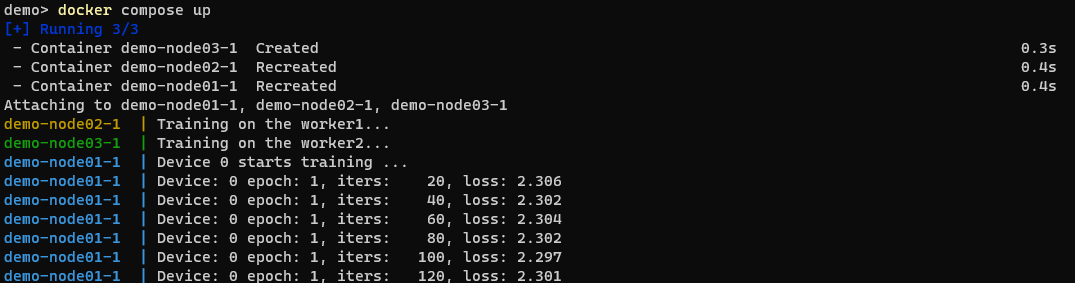
\includegraphics[width=1\textwidth]{figures/task4-docker-compose-up.png}
	\caption{caption:task4-docker-compose-up}
	\label{fig:task4-docker-compose-up}
\end{figure}


关于RPC的使用,助教总结的十分有限,还请同学们见谅。因此因此关于本章的的更多内容,还请同学们参考教程和文档。

\begin{itemize}
    \item 教程Distributed RNN using Distributed Autograd and Distributed Optimizer:\url{https://pytorch.org/tutorials/intermediate/rpc_tutorial.html#distributed-rnn-using-distributed-autograd-and-distributed-optimizer}
    \item rpc文档:\url{https://pytorch.org/docs/stable/rpc.html}
\end{itemize}





